% This work is made available under the terms of the
% Creative Commons Attribution-ShareAlike 4.0 license,
% http://creativecommons.org/licenses/by-sa/4.0/.

\chapter{Associations}
\label{associations}

Associators in WEKA are very limited in terms what you can do with them: you
can build an associator and output its rules, it the algorithm supports it.
The flow\footnote{adams-weka-associator.flow} in Figure \ref{associator}
shows how to train an associator using the \textit{WekaTrainAssociator}
transformer, which uses the Apriori setup obtained from the \textit{WekaAssociatorSetup}
source, and outputs the Apriori model and the rules that Apriori generated.

\begin{figure}[htb]
  \centering
  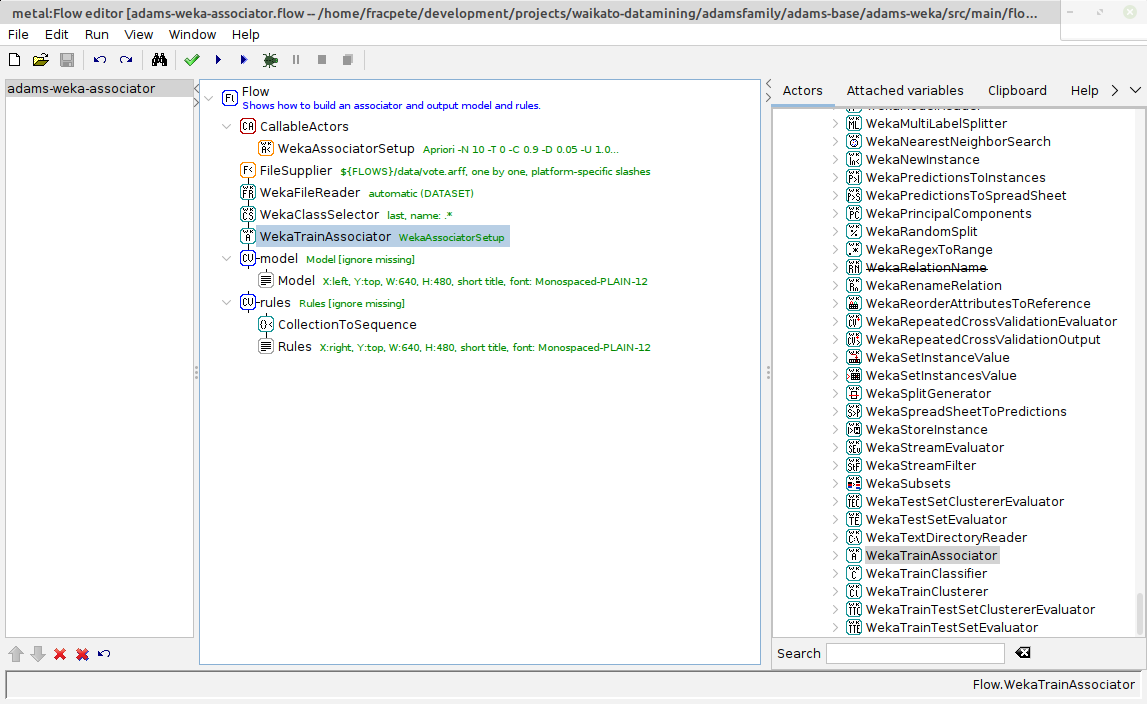
\includegraphics[width=12.0cm]{images/associator.png}
  \caption{Flow for building an associator and outputting model and rules.}
  \label{associator}
\end{figure}
